\documentclass[a4paper,12pt]{article}

\usepackage[utf8]{inputenc} % spécifie l'encodage du fichier
\usepackage[english,francais]{babel} % permet de traduire les éléments latex (date, titres de sections, etc.)

\usepackage{geometry} %
\geometry{a4paper}

\usepackage{graphicx}
\usepackage{float}
\graphicspath{{tests/}}

\usepackage{array}

\usepackage[hidelinks=true]{hyperref}

\usepackage{pdfpages}
\usepackage{listings}


\usepackage{fancyhdr}
\pagestyle{fancy} 

\linespread{1.5}

\fancyhead[R]{\rightmark}
\fancyhead[L]{\leftmark}
\renewcommand{\footrulewidth}{1pt}

\begin{document}

\includepdf[pages=last-last]{dev2}

\begin{titlepage}
\selectlanguage{francais}

\newcommand{\HRule}{\rule{\linewidth}{0.5mm}}

\begin{center}

\textsc{\LARGE Programmation parallèle haute performance\\[1.5cm] 
\textsc{\Large Travail pratique \#2 - INF7235 (gr. 10)}}\\[0.5cm]
\textsc{\large Hiver 2014}\\[0.5cm] 

\HRule \\[0.4cm]
{ \huge \bfseries Parallélisation en MPI/C d'une méthode Monte-Carlo appliquée à un jeux de hasard }\\[0.4cm] % Titre de votre document
\HRule \\[1.5cm]

\end{center}


\begin{minipage}{0.4\textwidth}
\begin{flushleft} \large
\emph{Auteurs:}\\
Johann \textsc{Dubois} % Nom de l'étudiant
\\
Clément \textsc{De Figueiredo}
\end{flushleft}
\end{minipage}

~~\\

\begin{center}
{\large \today}\\[3cm] % Date: \today insère la date du jour actuel

\vfill

\end{center}

\end{titlepage}
\newpage % nouvelle page

\tableofcontents % Génération du sommaire


\renewcommand\thesection{\Roman{section}}

\newpage % nouvelle page


\section{Description du problème}

"\textit{Le terme méthode de Monte-Carlo, ou méthode Monte-Carlo, désigne toute méthode visant à calculer une valeur numérique en utilisant des procédés aléatoires, c'est-à-dire des techniques probabilistes.}" \cite{wiki:montecarlo}
\\
Dans le programme élaboré dans le cadre d'un travail de session pour le cours de programmation parallèle haute performance, la méthode de Monte-Carlo est appliquée aux jeux de hasard.
Plus précisément, c'est le jeu du Loto qui a été choisi afin d'y appliquer la méthode de Monte-Carlo. En effet, l'objectif est de savoir quelles sont les probabilités qu'un nombre apparaisse plus qu'un autre. Dans ce but, plusieurs techniques de parallélisme ont été mise en place et leurs performances ont été mesurées afin de connaître quelle était la meilleure approche dans le contexte de la méthode de Monte-Carlo appliquée au jeu du Loto. 


\section{Approches utilisées}

\subsection{Implémentation de Monte-Carlo}
Le langage choisit afin d'utiliser la librairie \textbf{MPI} et le langage \textbf{C}. Ce langage a été choisi car la librairie \textbf{MPI} est compatible avec ce langage et nous disposions de connaissances suffisante en \textbf{C} afin d'implémenter cette solution de Monte-Carlo. 
\\\\Dans un premier temps, MPI est initialisé avec \textbf{MPI\_Init} puis les processus esclaves sont identifiés avec l'instruction \textbf{MPI\_Comm\_rank}. Ensuite, si le processus actuel est le processus maître alors divers opérations sont effectuées : séquentielle, parallèle statique et parallèle dynamique (sac de tâches). Chaque temps d'exécution des divers calculs sont stockés grâce à la variable \textbf{MPI\_Wtime} et sont affichés à la fin d'exécution du programme.

\subsection{Génération de nombres aléatoires}
La génération du nombre aléatoire utilisé dans la cadre de la fonction de tirage au sort a été faite de façon « Thread Safe ». C'est-à-dire que cela prévient les problèmes d'exclusion mutuelle qui pourrait avoir lieu si 2 threads voudraient récupérer une valeur, car la méthode de génération aléatoire se base sur l'horloge pour proposer un nombre.\\\\
L'utilisation de nombres aléatoires en C se fait avec les fonctions \textit{srand()} et \textit{rand()}. La première prend un argument qui servira de graine pour la génération de nombre. L'idée est alors de fournir une valeur de temps couplé avec le numéro du thread pour que la valeur soit différente pour chaque processus. \\
Le code suivant nous donne alors une valeur aléatoire « Thread Safe » : \\
\textit{srand(time(NULL) {\large \textasciicircum}  numProc);}


\subsection{Versions parallèles}

\subsubsection{Statique}
La version parallèle statique correspond à une version parallèle à granularité fine avec association statique entre tâches et threads. Autant de tâches vont être créées qu'il y a de processeurs. Chaque processus fait effectuer le tirage et les résultats vont être stockés localement. Ensuite, l'instruction \textbf{MPI\_Reduce} va avoir pour rôle d'effectuer une réduction et d'additionner (grâce à l'argument \textbf{MPI\_SUM}) tous ces résultats entre eux, le résultat final étant stocké dans un tableau final. Pour finir, on affiche les données issues du tableau récapitulatif ainsi que le temps d'exécution total. 

\subsubsection{Dynamique}
La version parallèle dynamique correspond à une version parallèle avec association dynamique entre tâches et threads de type « sac de tâches ». Cette version réalise la même opération que la version statique cependant quelques différences sont présentes. Un processus maître appelé « Coordinateur » a pour rôle de distribuer les tâches aux différents processus appelés « travailleurs ». Les « travailleurs » reçoivent les différentes tâches à effectuer avec l'instruction 

\section{Résultats expérimentaux}

\subsection{Application de test}
L'application doit être compilée et lancée avec au moins la version 4.4.7 de \textbf{gcc} (présent sur le cluster Turing de l’UQAM). Un makefile est également fourni afin d'exécuter les différentes versions du programme.\\\\
Les commandes disponibles dans le makefile sont les suivantes :
\begin{itemize}
	\item{\textbf{make compile}} (comportement par défaut de l'instruction make) pour compiler le code source
	\item{\textbf{make tests}} afin de vérifier le bon fonctionnement du programme
	\item{\textbf{make mesures}} pour exécuter le programme et en mesurer les performances
\end{itemize}~~\\
Des variables d'exécution pour également être modifiées. La variable \textbf{I} correspond au nombre total d'itérations effectués par la fonction \textbf{tirage} ainsi que la variable \textbf{NP} qui indique le nombre de processeurs utilisé par le programme.


\subsection{Conditions des tests}
Pour réaliser différents tests, plusieurs valeurs différentes vont être testées dans un environnement identique afin que les mesures soient comparables. L'application étant dépendante de la génération de nombre aléatoire, c'est pourquoi chaque mesure a été effectuée cinq fois et la moyenne de ces cinq tests a été retenue comme valeur finale. 

\subsection{Résultats}
Afin d'étudier les effets d'une implémentation parallèle, nous avions varié trois paramètres : le nombre d'itérations du tirage au sort, le nombre de threads et le nombre de tâches. \\
Dans les résultats présentés par la suite, \textit{S} correspond à « séquentiel », \textit{PS} à « parallèle statique » et enfin \textit{PD} à « parallèle dynamique ». 

\subsubsection{Variation du nombre d'itérations}
La méthode de Monte-Carlo consiste à réaliser un grand nombre de fois une opération pour que la probabilité qu’un certain nombre soit choisi soit élevée, dans le cas de notre application de la méthode au jeu de Loto. Nous allons donc faire varier la valeur correspondante aux itérations du calcul sur une échelle allant de dix à cents millions (Tab. \ref{tab:tempsexec1} et Fig. \ref{fig:tempsexec1}).\\

\begin{table}[H]
\caption{Résultat de la variation de la répétition}
\label{tab:tempsexec1}
\begin{tabular}{|l|l|l|l|l|l|l|l|l|}
\hline
            & \textbf{10} & \textbf{100} & \textbf{1000} & \textbf{10000} & \textbf{100000} & \textbf{1000000} & \textbf{10000000} & \textbf{100000000} \\ \hline
\textbf{S}  & 0,000       & 0,001        & 0,001          & 0,009           & 0,084           & 0,818              & 5,125               & 47,876               \\ \hline
\textbf{PS} & 0,003       & 0,001        & 0,001          & 0,003           & 0,021           & 0,206              & 1,973               & 20,189               \\ \hline
\textbf{PD} & 0,005       & 0,002        & 0,003          & 0,005           & 0,031           & 0,181              & 1,827               & 18,003               \\ \hline
\end{tabular}
\end{table}

\begin{figure}[H]
\center 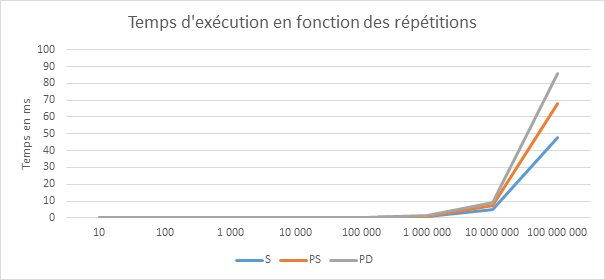
\includegraphics[width=15cm]{exec1}
\caption{Temps d'exécution en fonction des répétitions}
\label{fig:tempsexec1}
\end{figure}

On observe que le temps d'exécution est sensiblement le même entre les trois versions jusqu'à un million de répétitions (entre 0 et 10 millisecondes). Une fois ce seuil franchi, le temps d'exécution augmente plus rapidement en séquentiel qu'en parallèle. Pour ce qui est de l'accélération, les versions statique et dynamique sont presque pareilles à un détail près. L'accélération de la version dynamique va continuer à croitre jusqu'à un million d'itérations là où l'accélération de la version statique va commencer à décroitre vers cents mille itérations (Tab. \ref{tab:acc1} et Fig. \ref{fig:acc1}).

\begin{table}[H]
\caption{Résultat de l'accélération avec la variation de la répétition}
\label{tab:acc1}
\begin{tabular}{|l|l|l|l|l|l|l|l|l|}
\hline
            & \textbf{10} & \textbf{100} & \textbf{1000} & \textbf{10000} & \textbf{100000} & \textbf{1000000} & \textbf{10000000} & \textbf{100000000} \\ \hline
\textbf{PS} & 0,000       & 1,111        & 0,900         & 3,107          & 4,038           & 3,970            & 2,598             & 2,371              \\ \hline
\textbf{PD} & 0,000       & 0,476        & 0,346         & 1,611          & 2,727           & 4,511            & 2,805             & 2,659              \\ \hline
\end{tabular}
\end{table}

\begin{figure}[H]
\center 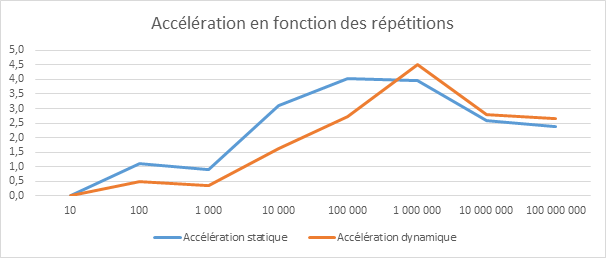
\includegraphics[width=15cm]{acc1} % image
\caption{Accélération en fonction des répétitions}
\label{fig:acc1}
\end{figure}

\subsubsection{Variation du nombre de processus}
Ce deuxième test consiste à faire varier le nombre de processus sur lequel/lesquels l'application va s'exécuter. Des valeurs vont être choisi allants de un à deux–cents avec des paliers de vingt-cinq. On peut voir que la méthode statique est légèrement plus rapide que la méthode dynamique. Au notera aussi qu'il n'y a aucun résultat pour la méthode dynamique lors de l'exécution du programme sur un processus. En effet, la mise en place d'une stratégie coordonnateur/travailleurs implique obligatoirement au moins 2 processus, ce qui explique le manque de résultat pour 1 processus (Tab. \ref{tab:tempsexec2} et Fig. \ref{fig:tempsexec2}).

\begin{table}[H]
\caption{Résultat de la variation du nombre de processus}
\label{tab:tempsexec2}
\begin{tabular}{|l|l|l|l|l|l|l|l|l|l|}
\hline
            & \textbf{1} & \textbf{26} & \textbf{51} & \textbf{76} & \textbf{101} & \textbf{126} & \textbf{151} & \textbf{176} & \textbf{201} \\ \hline
\textbf{S}  & 0,079      & 0,083       & 0,086       & 0,089       & 0,093        & 0,095        & 0,180        & 0,181        & 0,200        \\ \hline
\textbf{PS} & 0,080      & 0,007       & 0,012       & 0,016       & 0,015        & 0,022        & 0,024        & 0,030        & 0,037        \\ \hline
\textbf{PD} & -          & 0,020       & 0,039       & 0,063       & 0,054        & 0,029        & 0,054        & 0,049        & 0,087        \\ \hline
\end{tabular}
\end{table}

\begin{figure}[H]
\center 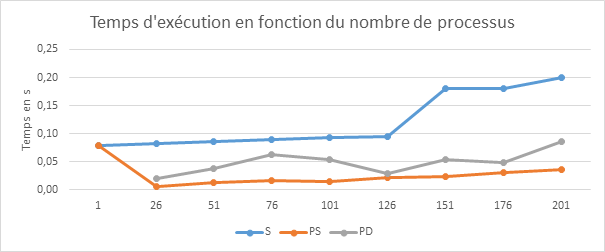
\includegraphics[width=15cm]{exec2}
\caption{Temps d'exécution en fonction du nombre de processus}
\label{fig:tempsexec2}
\end{figure}

La mesure d'accélération montre bien que la version statique est plus efficace que la version dynamique, surtout à partir de vingt-six processus. Cependant, les valeurs d'accélération ont tendances à se rapprocher vers cent vingt-six processus (Tab. \ref{tab:acc2} et Fig. \ref{fig:acc2}).

\begin{table}[H]
\caption{Résultat de l'accélération avec la variation du nombre de processus}
\label{tab:acc2}
\begin{tabular}{|l|l|l|l|l|l|l|l|l|l|}
\hline
            & \textbf{1} & \textbf{26} & \textbf{51} & \textbf{76} & \textbf{101} & \textbf{126} & \textbf{151} & \textbf{176} & \textbf{201} \\ \hline
\textbf{PS} & 0,990      & 12,831      & 6,895       & 5,547       & 6,393        & 4,338        & 7,500        & 5,960        & 5,405        \\ \hline
\textbf{PD} & -          & 4,212       & 2,204       & 1,422       & 1,733        & 3,276        & 3,333        & 3,686        & 2,299        \\ \hline
\end{tabular}
\end{table}

\begin{figure}[H]
\center 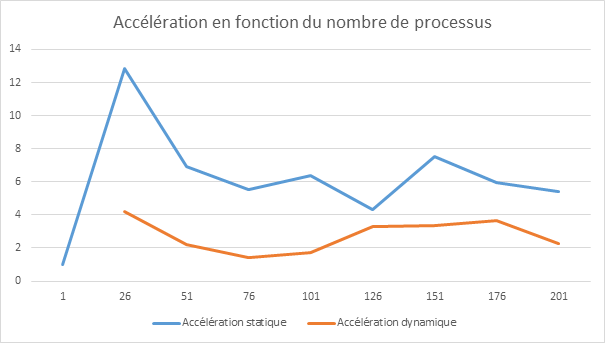
\includegraphics[width=15cm]{acc2} % image
\caption{Accélération en fonction du nombre de processus}
\label{fig:acc2}
\end{figure}


\subsubsection{Variation du nombre de tâches}
%qd ntache => repetition : c'est une version séquentiel car 1 seul proc travail
Dans la version parallèle dynamique de notre implémentation de la méthode de Monte-Carlo, on divise le nombre de tâches en plusieurs groupes pour que chaque thread réalise une tâche après l'autre jusqu'à la fin de la queue. Chaque thread récupère une tâche lorsque sa tâche précédente est terminée, dans le cas contraire il attend une opération de communication afin de transmettre ces résultats au thread maître. \\
Nous allons donc tester différentes valeurs allant de dix tâches à cent millions de tâches afin d'observer les effets de la variation d'un petit ou grand nombre de tâche sur les différentes versions du programme.\\
Comme prévu, les résultats ne varient pas avec les méthodes séquentielle et statique car le nombre de tâche est fixe au contraire de la version dynamique. On peut donc voir que la version dynamique est plus performante que la version séquentielle entre 100 et 100 000 tâches, mais une fois que le découpage de tâche est égale ou supérieur au nombre d'itérations, un seul thread travail car il n'y a qu'une grosse tâche, ce qui rend cette version identique à une version séquentielle (Tab. \ref{tab:tempsexec3} et Fig. \ref{fig:tempsexec3}). 

\begin{table}[H]
\caption{Résultat de la variation du nombre de tâches}
\label{tab:tempsexec3}
\begin{tabular}{|l|l|l|l|l|l|l|l|l|l|}
\hline
            & \textbf{10} & \textbf{100} & \textbf{1000} & \textbf{10000} & \textbf{100000} & \textbf{1000000} & \textbf{10000000} & \textbf{100000000} \\ \hline
\textbf{S}  & 0,080        & 0,080        & 0,079       	 & 0,079         & 0,079          & 0,079           & 0,079            & 0,079             \\ \hline
\textbf{PS} & 0,021       & 0,021        & 0,021         & 0,021          & 0,022           & 0,021            & 0,023             & 0,025              \\ \hline
\textbf{PD} & 0,571       & 0,057        & 0,031         & 0,034          & 0,082           & 0,082 & 0,082 & 0,082              \\ \hline

\end{tabular}
\end{table}

\begin{figure}[H]
\center 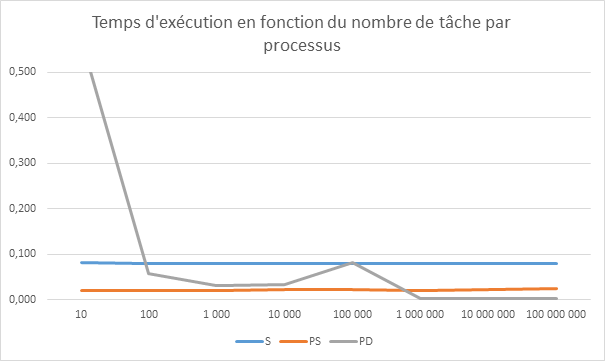
\includegraphics[width=15cm]{exec3}
\caption{Temps d'exécution en fonction du nombre de tâches}
\label{fig:tempsexec3}
\end{figure}

Afin de mieux observer les résultats, voici le calcul de l'accélération des deux méthodes parallèles. On aperçoit bien que la version dynamique est performante quand le découpage des tâches est inférieur au nombre de répétitions, bien que si les tâches sont trop petites l'accélération est en dessous de 1 ce qui signifie qu'elle n'est pas optimisée (Tab. \ref{tab:acc3} et Fig. \ref{fig:acc3}). 


\begin{table}[H]
\caption{Résultat de l'accélération avec la variation du nombre de tâches}
\label{tab:acc3}
\begin{tabular}{|l|l|l|l|l|l|l|l|l|l|}
\hline
            & \textbf{10} & \textbf{100} & \textbf{1 000} & \textbf{10000} & \textbf{100000} & \textbf{1000000} & \textbf{10000000} & \textbf{100000000} \\ \hline
\textbf{PS} & 3,903       & 3,813        & 3,845          & 3,726          & 3,563           & 3,766            & 3,433             & 3,169              \\ \hline
\textbf{PD} & 0,141       & 1,389        & 2,555          & 2,324          & 0,971           & 0,956 			& 0,964             & 0,961            	 \\ \hline

\end{tabular}
\end{table}

\begin{figure}[H]
\center 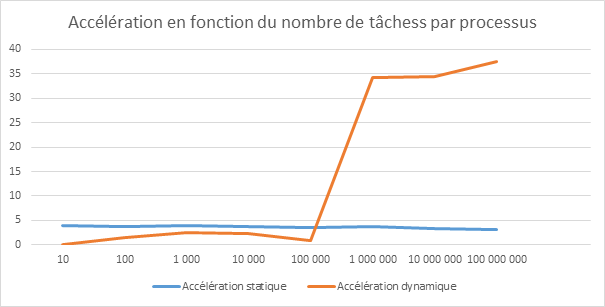
\includegraphics[width=15cm]{acc3} % image
\caption{Accélération en fonction du nombre de tâches}
\label{fig:acc3}
\end{figure}

\subsection{Analyse}
Pour l'analyse des résultats, nous nous sommes basés sur les valeurs de obtenus lors des calculs d'accélérations afin de savoir quelles sont les versions du programme qui sont les plus efficaces. 
\\\\
\indent D'une part, on observe que lorsqu'on varie le nombre d'itérations du calcul, le gain en temps d'exécution est sensiblement le même pour les trois méthodes jusqu'à cent mille d'itération. Passer cette valeur, on peut observer une accélération de la part des versions parallèles pouvant aller jusqu'à 4,5 fois plus rapide (version dynamique) pour un million d'itération. On utilisera donc les versions parallèles pour des itérations supérieures à mille fois l'opération de tirage. 
\\\\
\indent D'autre part, lorsqu'on varie le nombre de processus, les versions parallèles sont tout de suite beaucoup efficaces. En effet, la version statique possède déjà une accélération de 26 lors de l'exécution du programme sur vingt-six processeurs et la version dynamique, quant à elle, est quatre fois plus rapide que la version séquentielle. Cette accélération va décroitre par la suite et restera entre quatre et huit par la version statique, et entre 2 et 4 pour la version dynamique. Encore ici, on peut conclure, que les versions parallèles sont plus performantes lors de l'exécution du programme sur de multiple processus et ceci est d'autant plus vrai pour la version statique. 
\\\\
\indent Enfin, lorsqu'on varie le nombre de tâches attribués par processus, on observe que les versions parallèles sont encore une fois plus performantes. Plus précisément, la version dynamique commence à être plus performante à partir de cent tâches et voit ensuite son accélération réduite jusqu'à arriver à une valeur nulle à partir de cent mille tâche. Pour la version statique, cette dernière est nettement plus efficace avec une accélération de presque quatre pour dix tâche qui va décroître ensuite doucement pour arriver à un peu plus de trois pour cent million de tâches.
\\\\
\indent Pour conclure, les versions parallèles sont plus performantes dans les trois cas présentés ci-dessus, mais les deux versions restent pour autant assez proches. Toutefois, la version dynamique se trouve moins performante dans le cas d'une répartition de tâches trop nombreuses par processus. Au vu de l'implémentation du problème, qui actuellement a pour but de résoudre un problème de taille fixe (six numéro différents du jeu de Loto), il aurai été intéressant de voir également les effets d'une variation de la taille du problème à résoudre et voir en quoi cela aurait un impact sur les différentes versions en terme de vitesse d'exécution et d'accélération. 


\newpage

\nocite{*} % permet d'afficher toutes les références sans qu'elles soient citées
\bibliographystyle{unsrturl}
\bibliography{biblio}

\end{document}
